In the previous section, time was supposed to be continuous. In this new chapter however, we will regard time as a discrete variable meaning that we consider fixed size time intervals for our inventory management study. To each of these periods corresponds a certain demand, denoted $d_i$ for period $i$, and a decision (called "action") that we take in order to satisfy the demand, denoted $a_i$. We represent this situation with plots similar to figure (\ref{periodic:plot}) where each box stands for a period of time. The question we have to answer in this chapter is : "What actions do I have to take in order to fulfill the demand minimizing the total cost ?", or similarly : "How many items $a_i$ should I buy in period $i$ to minimize the cost ?"

\begin{figure}[h!]
    \centering
    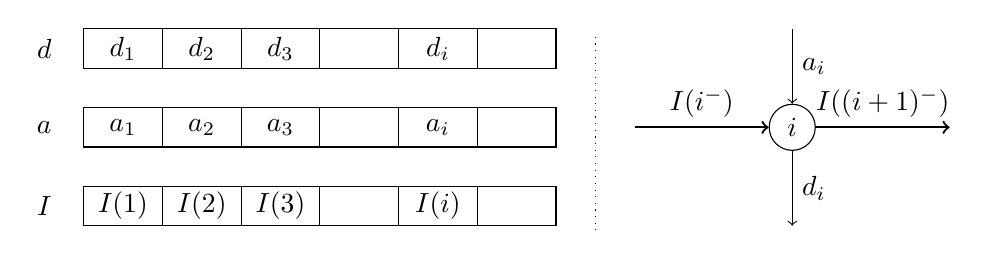
\begin{tikzpicture}
        \draw (.5, .25) node {$d$};
        \foreach \x/\t in {1/$d_1$, 2/$d_2$, 3/$d_3$, 4/$\hdots$, 5/$d_i$, 6/$\hdots$} {
            \draw (\x, 0) rectangle (\x+1, .5);
            \draw (\x+.5, .25) node {\t};
        }

        \draw (.5, -.75) node {$a$};
        \foreach \x/\t in {1/$a_1$, 2/$a_2$, 3/$a_3$, 4/$\hdots$, 5/$a_i$, 6/$\hdots$} {
            \draw (\x, -1) rectangle (\x+1, -.5);
            \draw (\x+.5, -.75) node {\t};
        }

        \draw (.5, -1.75) node {$I$};
        \foreach \x/\t in {1/$I(1)$, 2/$I(2)$, 3/$I(3)$, 4/$\hdots$, 5/$I(i)$, 6/$\hdots$} {
            \draw (\x, -2) rectangle (\x+1, -1.5);
            \draw (\x+.5, -1.75) node {\t};
        }

        \draw[dotted] (7.5, .4) -- ++(0, -2.5);

        \draw (10, -.75) node[circle, draw] (i) {$i$};
        \draw[->, thick] (8, -.75) -- node [above] {$I(i^-)$} (i);
        \draw[->] (10, .5) -- node [right] {$a_i$} (i);
        \draw[->] (i) -- node[right] {$d_i$} (10, -2);
        \draw[->, thick] (i) -- node[above] {$I((i+1)^-)$} (12, -.75);
    \end{tikzpicture}
    \caption{\label{periodic:plot}A representation of the periodic review model}
\end{figure}

With this representation, it becomes clear that, at the end of the $i$-th period, the inventory level, denoted by $I((i+1)^-)$, corresponds to the inventory level we had at the beginning of that period, $I(i^-)$, to which we should add the number of items we have ordered, $a_i$, minus the demand, $d_i$, which corresponds to goods which have been sold out. Hence, \[ I((i+1)^-) = I(i^-) + a_i - d_i \] Thus, by denoting by $h$ the inventory cost and by $K$ the fixed cost per order as we have been doing so far, the total cost can be computed as :
\[
    J = \sum_{i=1}^N\left( K\delta(i) + hI((i+1)^-) \right)
    \textrm{ where }
    \delta(i) = \begin{cases}
        1 &\textrm{ if } a_i > 0\\
        0 &\textrm{ otherwise }
    \end{cases}
\]

Our goal is to minimize this function by choosing relevant $a_i$s. For example, we need to discuss whether it is more profitable to order goods for two periods in a row instead or ordering period per period with respect to the demand. This can be solved by mixed integer linear programming models in an exact way. However, the cost of these methods are not worth it since efficient Heuristics have been developed which are very simple to implement. In this chapter, we will focus on the "Silver-Mill Heuristic". 

Even though it appears clear, note that, if the inventory level in period $0$ is $0$ and if we suppose knowing in advance the exact demand for each period, then it holds that \[ \sum_{i=0}^N a_i \ge \sum_{i=0}^Nd_i \]This can easily be demonstrated by recursivity. Let's suppose that $I_0=0$. Then, and because $I_i\ge 0, \forall i$ in the deterministic model, $I_1=a_1-d_1\ge 0$ which means that $a_1\ge d_1$. So the property is true for the first rank. Let's now suppose, that, for a given rank $k$, we have $\sum^k a_i\ge \sum^k d_i$. Considering $I_{k+1}$, it holds that $I_{k+1} = I_k + a_{k+1} - d_{k+1}$ with $I_k = \sum^k a_i - \sum^k d_i$ so that in definitive $\sum^{k+1}a_i\ge\sum^{k+1}d_i$.

\section{The Wagner-Within Theorem}

The Wagner-Within Theorem tells us about the shape of the solution to our problem. It stipulates that the optimal solution is either that (1) we buy exactely the demand of multiple time periods or (2) we buy exactely the current period demand, but in no case we would buy a fraction of the demand for one time period and buy the rest in another period. The optimal solution cannot be splitted into periods of time. For instance, the optimal solution cannot be to buy 70\% of the forecasted demand of November in September and 30\% of that same demand in October, but rather buy all the corresponding demand for November in September or all the corresponding demand for Novemeber in October. We do not split the orders for one time period. So that, considering $a_1$ for example, we now know that \[ a_1 \in \{ d_1, d_1+d_2, d_1+d_2+d_3, \hdots \} \] In this section we will demonstrate this theorem for the case of two time periods \WLOG. 

Let's consider a time horizon of two periods and, since the demand is supposed to be known in a deterministic way, we can impose that the inventory level at the end of the horizon is zero, $I_2=0$. As well, we'll assume that $I_0$ is zero (no initial inventory level). 

\section{The Silver \& Mill Heuristic}

\section{Analysis of the method}
